\chapter{Projekt języka}
\label{cha:wywodJezyka}
%jakieś podnagłówki
W literaturze definiuje się język jako podzbiór zbioru skończonych ciągów symboli nad pewnym alfabetem”\cite{hopcroft_automaty}. Definicją taka zachęca, aby dokonać z pozoru arbitralnego wyboru elementu tej przestrzeni podzbiorów i bez wyjaśnień opisać go, najlepiej w formie gramatyki bezkontekstowej, która to forma stała się praktycznym standardem w konstrukcji kompilatorów. Świadczy o tym definicja użyta w jednym z najważniejszych artykułów w dziedzinie translacji – „Parsowaniu języków od lewej, do prawej” Donalda Knutha z 1966\cite{TRANSLATION_FROM_LEFT_TO_RIGHT}, opisującej mechanizm, który dzisiaj nazywa się parserem LR. 
„The language defined by G is
\[
\{ \alpha \mid S \Rightarrow \alpha \text{ and } \alpha \text{ is a string over } T \}
\]
namely, the set of all terminal strings derivable from S by using the productions of G as substitution rules.”

W wolnym tłumaczeniu:
„język zdefiniowany przez gramatykę G to \[
\{ \alpha \mid S \Rightarrow \alpha \text{ i } \alpha \text{ to napis nad } T \}
\]czyli zbiór wszystkich ciągów terminali wyprowadzalnych z symbolu startowego S poprzez zastosowanie G jako zbioru produkcji”.

Powyższą definicja jest kontynuacją myśli wyrażonej jeszcze w 1926 roku przez Bloomfielda\cite{BLOOMFIELD_1926}, który poszukując pierwszej w zachodniej nauce formalizacji lingwistyki, chcąc wyzbyć się wszelkich odniesień do „mentalnych stanów”, uznawanych przez ówczesne poglądy za niemierzalne, a przez to nienadające się do budowy empirycznej nauki, skupił się jedynie na zewnętrznych, a przez to opisywalnych przejawach języka, a przez to jego zewnętrznej reprezentacji,  czyli ekstensji języka.\cite{parsing_timeline_kegler}

Wszelako poznanie „intensji” języka, czyli dobre zrozumienie koncepcji stojących za nim, zdaje się niezwykle pożyteczne, gdy konstruuje się jego translator. Istnieje pogląd, który Peter Naur, (przytoczony w tym miejscu bo właśnie on jest twórca powszechnej notacji gramatyk formalnych), wyraża w swym artykule „Programowanie jako budowanie teorii” – jakoby kod stanowił zaledwie mniejszą część programu, a większą i istotniejszą jest mentalny model w umyśle programisty go piszącego\cite{NAUR_1985}. Dlatego też spróbujemy wpierw osiągnąć pewne wyobrażenie o projektowanym języku, a dopiero potem ująć go formalnie. 

Sam proces projektowania nowych języków jawi się dość tajemniczo, ponieważ twórcy języków rzadko opisują go bezpośrednio. Czytamy jedynie o wnioskach wyciągniętych post factum – np. Dennis Ritchie stwierdził, że należało przyjąć inną precedencję operatorów || i \&\&\cite{Ritchie_mail}, czy w najlepszym wypadku stwierdzenia w rodzaju wygłoszonego przez Wirtha, że twórca języka powinien być ,,rozsądnym zbieraczem rozwiązań'' (judicious collector of features)\cite{Wirth_recollections_Pascal}. Z tego, co możemy dowiedzieć się z literatury, można złożyć obraz dwóch przeciwstawnych sobie kierunków, sił rywalizujących ze sobą przy projektowaniu języka:

Pierwszą jest pewien rodzaj pryncypium najmniejszych zaskoczeń, zwłaszcza w dzisiejszych czaszach, gdy języki wysokiego poziomu stały się powszechne i pewien ich kształt jest oczekiwany przez programistę, stanowiąc niemal lingua franca, i umożliwiając pobieżne czytanie nieznanych wcześniej acz spokrewnionych języków. Ująć to możną również  że każdy język wysokiego poziomu, a w szczególności imperatywny, zawrzeć musi w sobie interpretację
\begin{enumerate}[noitemsep, label=(\alph*)]
    \item Wyrażeń matematycznych
    \item Podstawowych struktur algorytmicznych
\end{enumerate}
na swój sposób musi zarazem być FORTRANEM – translatorem formuł matematycznych oraz ALGOLEM – językiem opisu algorytmów.
Wypełnienie tych dwóch oczekiwań wprowadza ustalone i dobrze poznane struktury gramatyczne do języka.

Przeciwstawna do chęci zaspokojenia oczekiwań ludzkiego umysłu, jest konieczność dostosowania się do technicznych możliwości parsera. Często to, co dla człowieka jest naturalne i czytelne, jest praktycznie niemożliwe do automatycznej analizy składniowej.  Sama teoria parsingu i jej dokładne ograniczenia jest zbyt złożona, aby ją przedstawić w takiej pracy, choć przegląd metod pojawi się przy opisie wybranego generatora parserów. Na szczęście, dwa wymienione metajęzyki (wyrażeń i prostych struktur algorytmicznych), doczekały się niezliczonych implementacji i gramatyki je opisujące są dobrze poznane. Zacznijmy zatem prostym przykładem
\begin{lstlisting}
dopóki(h>0)
{
    Dv = g * Dt - opór(v, h);
    v += Dv;
    jeśli( abs(Dv) < eps_Dv) {prędkość_graniczna = v;}
    h -= v * Dt;
}
jeśli(prędkość_graniczna == 0)
    {pisz("Nie wyznaczono prędkości granicznej");}
inaczej {pisz("Przybliżeniem prędkości granicznej jest %f, jeśli funkcja oporu aerodynamicznego ma pewne własności.");}
\end{lstlisting}


Obrazuje to chyba dość dobrze oczekiwania wobec dowolnego języka imperatywnego – niezależnie od szczegółów, proste pętle, warunki i wyrażenia matematyczne (lub fizyczne) zawsze będą wyglądać podobnie, nawet jeśli wychodzilibyśmy od składni języka innego niż C. (A przynajmniej będą dostępne łatwo rozpoznawalne wersje podstawowych struktur kontroli przepływu - wiele jest form i semantyk instrukcji \textit{for} w różnych językach, lecz po \textit{while} można się spodziewać niemal zawsze tego samego.)

O ile zapis wywołania funkcji ma postać ustaloną powszechnym oczekiwaniem (oraz matematyką), o tyle więcej możliwości pojawia się przy jej deklaracji.
\begin{lstlisting}
rzeczywista opór(rzeczywista v, h)
{
	zwróć -6*PI*v^2*M*R;
}
\end{lstlisting}

\begin{lstlisting}
fun  opór(rzeczywista v, h) -> rzeczywista
{
	zwróć -6*PI*v^2*M*R; //formuła Stokesa
}
\end{lstlisting}
\begin{lstlisting}
opór = lambda v,h: -6*PI*v^2*M*R;\end{lstlisting} - jeśli gotowi jesteśmy na implementację inferencji typów.
albo nawet 
\lstset{
    escapechar=|,
    breaklines=true
}
\begin{lstlisting}
opór = |$\lambda$| v.h. -6*PI*v^2*M*R\end{lstlisting} – jeśli chcemy zmuszać użytkownika do zaopatrzenia się w grecką klawiaturę i złamać oczekiwania w kwestii semantyki kropki
\lstset{
    escapechar=@
    breaklines=true
}
\begin{lstlisting}
def f(x: int) -> int:               	 Python
function f(x: number): number { ... }    TypeScript
fun f(x: Int): Int { ... }          	 Kotlin
int f(int x) { ... }                	 C
auto f(int x) -> int { ... }        	 C++ (nowsza składnia)
int f(x int) { ... }                	 Go
f(x: int) -> int do ... end         	 Elixir
f(x :: Int) :: Int = ...            	 Haskell
function f(x) return x + 1 end      	 Lua
def f(x: Int): Int = ...            	 Scala
func f(x int) int { ... }           	 Go
public int f(int x) { ... }         	 Java
fun f(x: Int): Int = x + 1          	 Kotlin
let f x : int -> int = x + 1        	 OCaml
fn f(x: i32) -> i32 { ... }         	 Rust
Function f(x As Integer) As Integer 	 VB.NET
\end{lstlisting}
\lstset{
    escapechar=|,
    breaklines=true
}
Jeśli dobrze przyjrzymy się dostępnym opcjom, to spostrzeżemy, że wszystkie chyba możliwości zostały przetestowane w jakimś powszechnie dostępnym języku. Możemy umieszczać typ przed, jak i po nazwie parametru, używać różnych odmian słowa kluczowego fun/function, typu zwracane umiejscowić przed nazwą funkcji, lub po, parametry przekazywać przez wartość, referencję, nazwę et cetera - dla każdej rozsądnej kombinacji konstrukcji składniowych prawdopodobnie można by znaleźć język jej używający.
Czy zatem nic ciekawego nie pozostało do zrobienia z funkcjami, mimo że mamy niepowtarzalną okazję stworzenia własnej gramatyki? (jęz.)

\section{Wielokrotne punkty wejściowe}
Natrafiłem kiedyś na podręcznik do dawno wymarłego już języka PL/I i zacząłem przeglądać z pewnym zainteresowaniem, ponieważ jest on odległym przodkiem języka procedur bazodanowych w Postgresie. Zwróciła moją uwagę strona 196 z podręcznika\cite{plif} oraz następna.

% \begin{figure*}[hb]
%     \centering
%     \makebox[\textwidth]{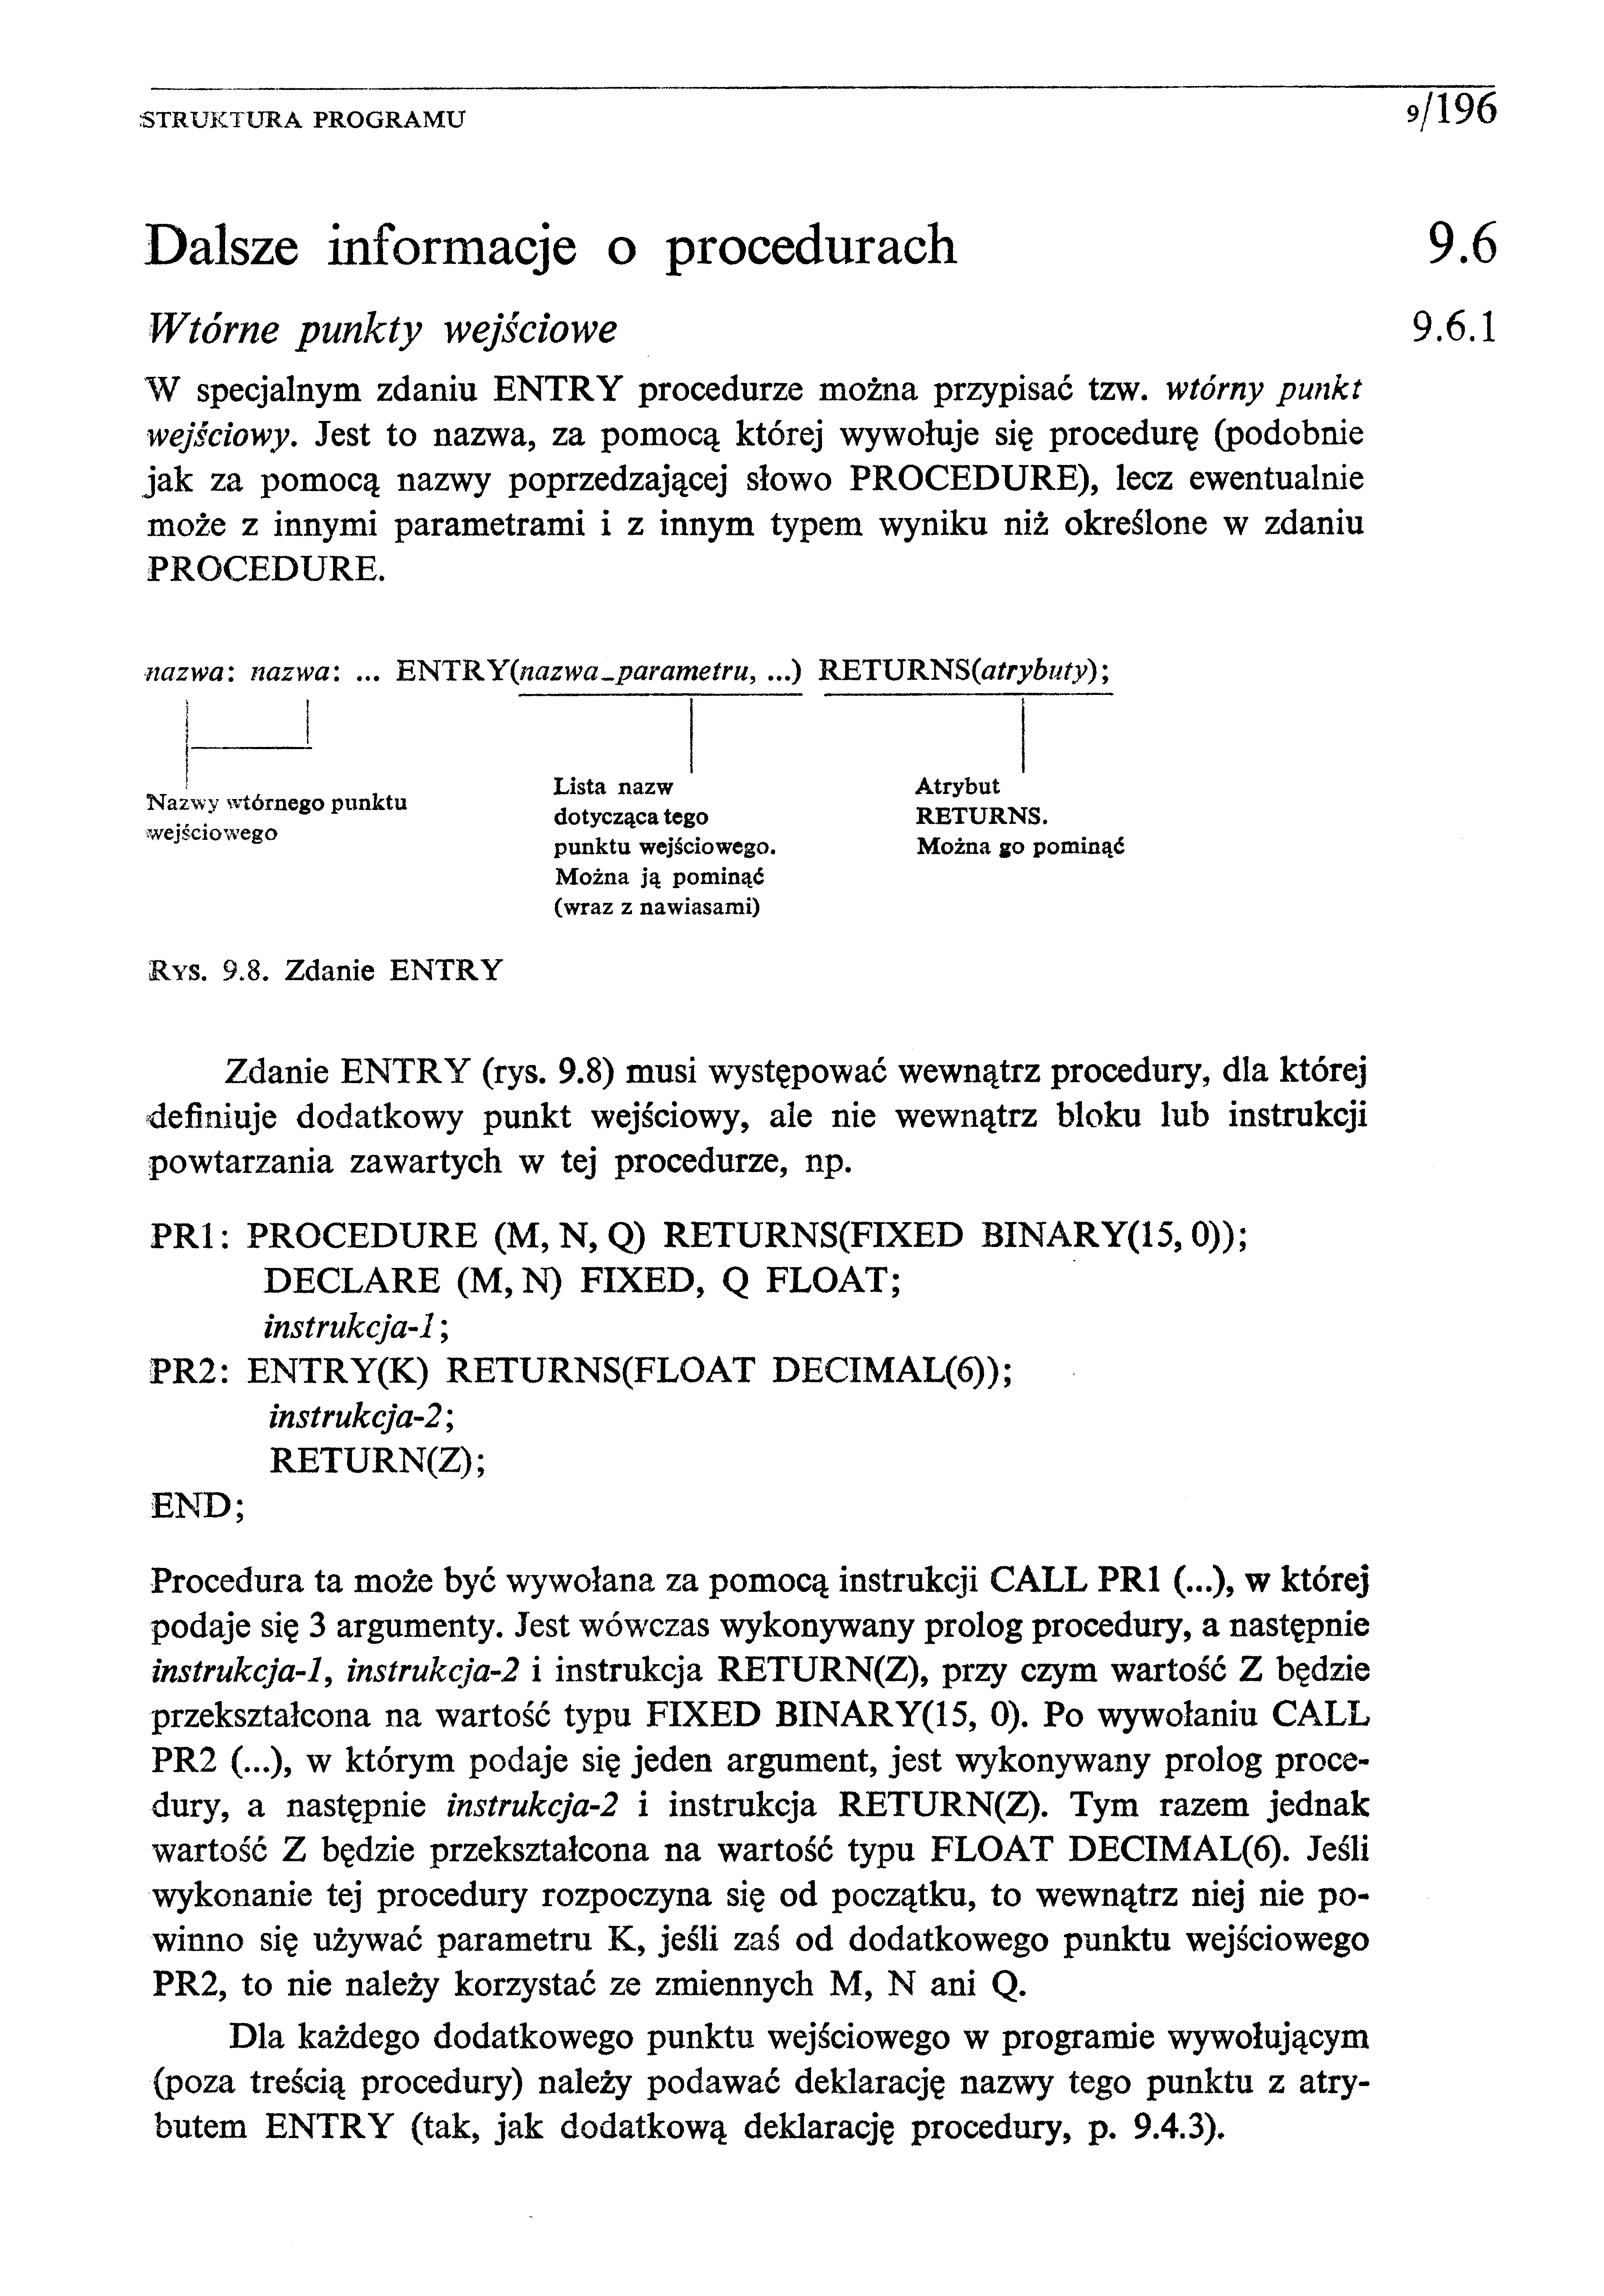
\includegraphics[width=.9\paperwidth]{images/wywod/PLI1_bin.png}}
%     \caption{Widok dekompilacji w programie GHIDRA}
% \end{figure*}
%[]
Przyjrzawszy się zamieszczonemu tam przykładowi, możemy skonstatować, że znamy obecnie znacznie poręczniejszą składnię argumentów domyślnych i należy pozostawić szybko za sobą ten drobny przypis do składni wymarłego języka. Ja wszak nie potrafiłem do końca zapomnieć o tej dziwacznej konstrukcji, nosząc przeświadczenie, że widziałem ją już wcześniej w innym miejscu. Systematyczna kwerenda ujawnia, że podobna składnia ze słowem kluczowym ENTRY pojawia się również w Fortranie\cite[str.~120]{bielecki}, oraz w COBOLU\cite{ibm_manual_on_ENTRY_in_COBOL}. Pewien czas wszakże upłynął, zanim znów przypadkowo dotarłem w miejsce, gdzie owo „entry” zobaczyłem po raz pierwszy -  na liście słów kluczowych C u Kernighana i Ritchiego, opatrzone wyjątkowo lakonicznym opisem, nie ujawniającym powiązanej z nim składni\cite[str.~120]{KiR}
W wydaniu drugim tej książki pojawia się stwierdzenie o wyłączeniu tego słowa kluczowego ze specyfikacji języka\cite[rozdz.~A2.4,~str.192]{KiR2}, odpowiadając już powszechnemu doświadczeniu C, jako języka pozbawionego takiej konstrukcji.

Szerzej zakrojone wysiłki w zakresie archeologii językowej, przedstawiają „ENTRY” i formy podobne, jako dziwaczne skamieliny – występujące powszechnie w pierwszym pokoleniu języków wysokiego poziomu, by potem stopniowo wymrzeć, poprzez zepchnięcie na marginesy standardów, zarzucenie, jak w C, czy zupełne zapomnienie, nie tylko przez programistów, lecz i projektantów języków w czasach późniejszych. W standardach i podręcznikach odbywa się to wymieranie bez obszerniejszych wyjaśnień, a w różnych mniej formalnych tekstach i urywkach, powtarzane są często opinie, jakoby konstrukcja ta miała być (jeszcze w latach 70) przestarzała, niezalecana,  passe, albo wręcz szkodliwa, otoczona aurą, charakteryzującą zazwyczaj rozwiązania wykorzystywane nagminnie w złych praktykach programistycznych. Przytoczę jeden przykład z forum (w odniesieniu do C):

„Really, it isn't a big loss. The concept of one subroutine with multiple entry points was on its way out even before C was new, and it was wise of the standards makers to ignore such a half-baked idea."\cite{delreth_on_entry}

„Naprawdę, to nie jest wielka strata. Koncepcja jednej procedury z wieloma punktami wejścia była w odwrocie jeszcze zanim C stał się nowy, i było mądre ze strony twórców standardów, że zignorowali tak niedopracowany pomysł.” (tłum.)
 
Nawet jeśli komentarze tego typu wygłaszane są przez programistów dość sędziwych, by pamiętać rzeczywiste uzasadnienie rezygnacji z pomysłu, uznają to za fakt dawno dokonany i uzasadniony, niestety nie dzieląc się szerszymi wyjaśnieniami na piśmie, przynajmniej nie dość często, by autor tej pracy je odnalazł. (Chociaż lektura wątku z \cite{delreth_on_entry} rzuca nieco światła na zagadnienie).
Nawet bez uzasadnień z epoki, można łatwo stwierdzić, że owa konstrukcja składniowa jest prostą konsekwencją przeniesienia sposobu pisania procedur wprost z języków niższego poziomu. Wyobraźmy sobie, że programista asemblerowy, w latach 60 napisał procedurę do drukowania zawartości tabeli. Krótka funkcja w C:

\begin{lstlisting}
void write_table(char *** cells, char ** colnames, int num_cols, int num_rows)
{
    for(int i=0; i<num_rows; i++)
    {
        if(i>0){putchar(',');}
        printf("%s", colnames[i]);
    }
    putchar('\n');
    for(int j=0; j<num_rows; j++)
    {
        for(int i=0; i<num_rows; i++)
        {
            if(i>0){putchar(',');}
            printf("%s", cells[j][i]);
        }
        putchar('\n');
    }
}
\end{lstlisting}

Przed językami wysokiego poziomu, byłaby obszerniejsza i mogłaby wyglądać tak:
(w celach demonstracyjnych użyto współczesnego asemblera NASM na architekture IA-32 (x86))

\begin{lstlisting}
write_table:
; Write column names
    xor eax, eax       ; Reset eax for loop variable
    mov ecx, num_cols  ; Number of column names to write
write_colnames:
    cmp eax, ecx       ; Compare current index with num_cols
    jge write_cells    ; If done, jump to write cells

    mov ebx, [colnames + eax * 4] ; Get pointer to current colname
    test eax, eax                 ; If index > 0
    jz .write_name                ; Skip comma on first colname
    mov esi, comma
    call write_string

.write_name:
    mov esi, ebx
    call write_string

    inc eax          ; Increment column index
    jmp write_colnames

write_cells:
    ; Loop through rows
    xor eax, eax      ; Row index
    mov edx, num_rows ; Total rows
row_loop:
    cmp eax, edx
    jge done          ; Exit after all rows are written
    push eax          ; Save row index

    ; Loop through cells in a row
    xor ecx, ecx      ; Reset column index
    mov esi, [cells + eax * 4] ; Get pointer to current row
write_row:
    cmp ecx, num_cols
    jge .next_row     ; Break when all cells in the row are written

    mov edi, [esi + ecx * 4] ; Pointer to cell
    test ecx, ecx
    jz .write_cell    ; Skip comma before first cell
    mov esi, comma
    call write_string

.write_cell:
    mov esi, edi
    call write_string

    inc ecx          ; Increment column index
    jmp write_row

.next_row:
    call write_newline
    pop eax          ; Restore row index
    inc eax
    jmp row_loop
\end{lstlisting}

Wyobraźmy sobie, że ta procedura ta używana jest wielokrotnie w istniejącym oprogramowaniu:
\begin{lstlisting}
...zapisywanie niektórych rejestrów (caller-save registers)
... ustawianie rejerestrów - argumentów
call write_table
...przywracanie rejestrów zapisywanych przez wołającego
\end{lstlisting}
Przypuśćmy, że pewnego dnia księgowy przychodzi do programisty utrzymującego to oprogramowanie i prosi, aby w dwóch z szesnastu przypadków użycia tej procedury, jednak nie drukować nagłówków. Dzisiaj lista parametrów funkcji write\_table zwyczajnie powiększyłaby się o flagę, określającą, czy pisać nagłówek. W asemblerze również można to zwięźle zapisać – dodać na początku procedury
\begin{lstlisting}
jz %rejestr_z_flagą write_cells
\end{lstlisting}
Trzeba jednak wtedy zmienić każde z wywołań procedury, jest to bardziej pracochłonne w języku niskiego poziomu, a jeśli argumenty są przekazywane w rejestrach, nie na stosie (co zdarza się w niektórych architekturach i dzisiaj), to konieczność znalezienia dodatkowego wolnego rejestru miejscu wywołania może zaburzyć ręcznie skonstrowany schemat przydziału rejestrów w okalającej procedurze. (A jak wspomniano, dowiedziono że problem przydziału rejestrów jest NP-zupełny.\cite{REGISTER_ALLOCATION_CHAITIN1981}) Dlatego dość prawdopodobne, że programista zwyczajnie w dwóch miejscach, zamiast
\begin{lstlisting}
call write_table
\end{lstlisting}
napisałby 
\begin{lstlisting}
call write_cells
\end{lstlisting}
write\_table i write\_cells są w istocie jedynie adresami i gdy nie ma rozbudowanego prologu procedury, można ją rozpocząć równie dobrze w innym punkcie w ten sposób. Możemy więc wyobrazić sobie, dlaczego programistom przywykłym do języków niskiego poziomu, taka konstrukcja wydałaby się naturalna:
\lstset{
    escapechar=|,
    breaklines=true
}
\begin{lstlisting}
void write_table(char *** cells, char ** colnames, int num_cols, int num_rows)
{
    for(int i=0; i<num_rows; i++)
    {
        if(i>0){putchar(',');}
        printf("%s", colnames[i]);
    }
    putchar('\n');
    
    |\textbf{entry}| write_cells(char *** cells, int num_cols, int num_rows);
    for(int j=0; j<num_rows; j++)
    {
        for(int i=0; i<num_rows; i++)
        {
            if(i>0){putchar(',');}
            printf("%s", cells[j][i]);
        }
        putchar('\n');
    }
}
\end{lstlisting}

Nie dziwi też, że takie relikty mogły być zwalczane, gdy próbowano wypracować i rozpowszechnić wśród praktyków, oczywiste dziś pojęcie funkcji, jako bloku kodu robiącego jedną rzecz, z paramtrami wejściowymi oraz wartością zwracaną. Inną konstrukcję bezpośrednio pochodzącą z asemblerów – goto rugowano bardzo długo, ochoczo i niemal z całkowitym sukcesem, podobnie jawne etykiety do niej potrzebne, składniowo skopiowane bezpośrednio z asemblerów. Czy może mieć dla nas ów zabytek paleografii jakiekolwiek znaczenie? Zauważmy, że opisuje on ciekawy byt: funkcja ma z algorytmicznego punktu widzenia jedno wejście i wiele wyjść, on ma zarówno wiele wyjść, jak i wejść.
\begin{figure}[h]
    \centering
    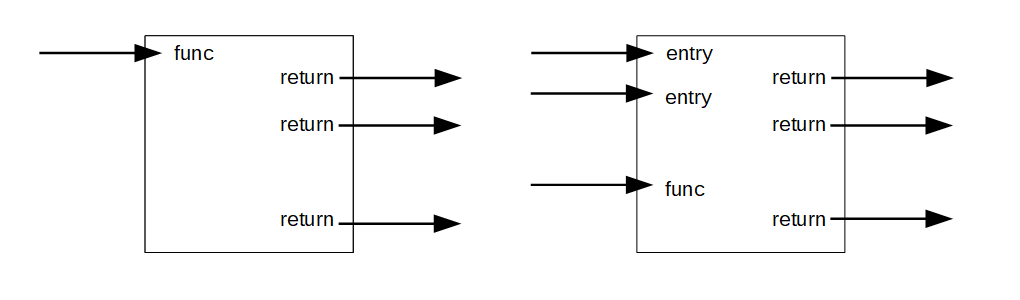
\includegraphics[width=0.6\textwidth]{images/wywod/pudelka.png}
    \caption{Funkcja z jednym punktem wejściowym a procedura z wieloma}
\end{figure}

Wszystkie historyczne implementacje wyróżniają jeden – główny oraz zero lub więcej punktów wejściowych, co zawsze wygląda dość podobnie:
\lstset{
    escapechar=|,
    breaklines=true
}
\begin{lstlisting}
|\textbf{pisz\_tabelę}|(znak ^^^ krotki,znak ^^ nazwy_kolumn, całk liczba_kolumn, całk liczba_wierszy)
{
    dla(całk i=0; i<liczba_wierszy; i++)
    {
        jeśli(i>0){putchar(',');}
        printf("%s", colnames[i]);
    }
    putchar('\n');
    
    |\textbf{wejście}| pisz_krotki(znak ^^^ krotki, całk liczba_kolumn, całk liczba_wierszy);
    dla(całk j=0; j<liczba_wierszy; j++)
    {
        dla(całk i=0; i<liczba_wierszy s; i++)
        {
            jeśli(i>0){putchar(',');}
            printf("%s", cells[j][i]);
        }
        putchar('\n');
    }
}
\end{lstlisting}
W ramach eksperymentu wznieśmy hasło: „Równe prawa dla wszystkich punktów wejściowych!”, przesuńmy nawiasy,  zamieńmy słowo kluczowe „wejście” na krótszy odpowiednik i otoczmy całą procedurę odpowiednim nagłówkiem:
\begin{lstlisting}
procedura {
|\textbf{tu}| pisz_tabelę(znak ^^^ krotki,znak ^^ nazwy_kolumn, całk liczba_kolumn, całk liczba_wierszy) -> Nic;
    dla(całk i=0; i<liczba_wierszy; i++)
    {
        jeśli(i>0){putchar(',');}
        printf("%s", colnames[i]);
    }
    putchar('\n');
    
|\textbf{tu}| pisz_krotki(znak ^^^ krotki, całk liczba_kolumn, całk liczba_wierszy)->Nic;
    dla(całk j=0; j<liczba_wierszy; j++)
    {
        dla(całk i=0; i<liczba_wierszy s; i++)
        {
            jeśli(i>0){putchar(',');}
            printf("%s", cells[j][i]);
        }
        putchar('\n');
    }
}
\end{lstlisting}
Uzyskaliśmy w ten sposób dość oryginalną składnię, która nie jest już reliktem asemblerów, lecz organiczną częścią języka. Teraz będzie można eksperymentalnie sprawdzić, czy wielowejściowe procedury są rzeczywiście szkodliwe, lub kłopotliwe w praktyce, czy też da się je kreatywnie wykorzystać. Można rówież powiedzieć, że przypominamy w ten sposób programiście, że nie pracuje z matematycznymi funkcjami, które udają dobrze języki funkcyjne, lecz w prostym, imperatywnym i przede wszystkim proceduralnym języku, nie mającym wielkich ambicji względem abstrakcji matematycznych.

Implementacja tej formy w gramatyce bezkontekstowej jest prosta: nieterminal sygnatury funkcji poprzedzamy słowem kluczowym i traktujemy jak jedną z instrukcji, na równi z np. warunkiem, czy pętlą, (zob. nieterminal instrukcja\_wkroczenia w gramatyce zamieszczonej w \ref{sect:gramatyka}).

\section{System typów}
W poprzednich przykładach niepostrzeżenie pojawiły się nazwy typów. „Typ określa możliwe operacje na bitach oraz uzgodnienia [konwersje] jakie wolno na nich stosować”\cite[str.~259]{waite_goos}. Język wysokiego poziomu nie może obejść się bez spójnego systemu typów, gdyż sprawdzanie ich jest jedną z głównych aspektów analizy semantycznej programu, typy niekiedy sterują też procesem przekładu.

Na system typów składa się zbiór typów podstawowych (atomicznych), zbiór konstruktorów typów, czyli reguł łączenia ich w typy złożone (np. struktur, tablic, czy funkcji – typy „strzałkowe”), oraz określenie operacji na nich dozwolonych, w tym specjalnych unarnych operacji do konwersji pomiędzy typami.
\begin{lstlisting}
całkowite x = 0;
x = y + 7.0;
\end{lstlisting}
Mając pewne użycie operacji $f$, (funkcji, lub operatora), oraz n-elementową krotkę użytych argumentów: $(t_1, t_2, ..., t_n)$, trzeba dysponować mechanizmem określającym, czy dane typy są dozwolone dla tej operacji. W bardziej skomplikowanych przypadkach, gdy istnieje wiele operacji o tej samej nazwie, stanowiących przeładowania nazwy lub operatora, mechanizm kompilatora musi wybrać właściwe dopasowanie argumentów do parametrów formalnych, spróbować dobrać odpowiednie konwersje automatyczne, lub zgłosić zrozumiały błąd.
W powyższym przykładzie, programista spodziewa się, że druga linia zostanie przetłumaczona bez zastrzeżeń, gdyż przywykł do oglądania takich napisów w kontekście matematycznym (fizycznym). Wymaga to wszak zastosowania różnych automatycznych konwersji, w zależności od typu zmiennej y.
\begin{lstlisting}
całkowite y; => x = całkowita(rzeczywista(y) + 7.0); 
                    lub
                x = y + całkowita(7.0)
                
rzeczywiste y; => x = całkowita(y + 7.0)

znak y; => podobnie jak całkowita, lub błąd, 
        (zależnie od reguł konkretnego języka)

Typ strukturalny T => błąd
        (chyba, że zdefiniowano przeładowanie operatora + dla T, całk.)
\end{lstlisting}

Zagadnienie dobrego zaprojektowania systemu typów, przestaje być proste, gdy włączymy do niego wszystkie powszechnie używane mechanizmy – konwersje jawne i automatyczne, przeładowania nazw i operatorów, polimorfizm oraz typy parametryzowane. W szczególności te ostatnie wydają się tak skomplikowanym konceptem, że często okazują się wykraczać poza wyobrażenia ich twórców\cite{cpp_templates_turing_complete}\cite{taming_wildcards_java}, z pewnością zaś przekraczają możliwości tak małego projektu.
W warunkach tak ograniczonych, na początku rozwoju języka, właściwym pytaniem wydaje się być „Jaki jest najprostszy możliwy w tym wypadku system typów?” Odpowiedź zapewnia system typów maszyny docelowej - llvma, będący z kolei pierwotnie przystosowany do języków C i C++. Skopiujemy więc w zasadzie system typów C, próbując go wszakże możliwie uprościć.
Typy podstawowe podyktowane są nawet nie przez samo LLVM, lecz przez architektury sprzętu, dysponującego dziś rejestrami całkowitymi o długościach od bajtu do słowa maszynowego (32/64 bity) oraz rozmaitymi rejestrami zmiennoprzecinkowymi, przechowującymi 32 lub 64 bitowe  reprezentacje liczb zmiennoprzecinkowych podług standardu IEEE754. (Pomijamy rejestry wektorowe)
\begin{center}
\begin{tabular}{|c|c|c|}
\hline
\textbf{Projektowany język} & \textbf{LLVM} & \textbf{C/C++} \\ \hline
znak                        & i8       & char               \\ \hline
całkowita/całk              & i64      & long long int      \\ \hline
rzeczywista/rzecz           & f64      & double             \\ \hline
\end{tabular}
\end{center}

Ascetycznie opuszczamy na razie liczby bez znaku, oraz mając okazje tworzyć język od początku, bez wymogów kompatybilności wstecznej, ignorujemy kłopotliwą i niewiele wnoszącą w praktyce dychotomię liczb 32/64bitowych. (LLVM przetłumaczy poprawnie arytmetykę na liczbach 64bitowych również na rozkazy maszyny 32 bitowej, zajmować wszak będzie każda zmienna dwa rejestry, nie będzie to kod efektywny. W roku pisania tej pracy maszyny 32 bitowe są już wyraźną mniejszością)

Nie są to jednak wszystkie typy potrzebne do funkcjonalnego systemu. Konieczne są jeszcze tablice:
\begin{lstlisting}
rzecz^ tabl = nowe [17] rzecz;
\end{lstlisting}
Jako że LLVM posiada wbudowane malloc, kopiujemy składnię alokacji na stercie z C++, przesuwając jedynie liczbę żądanych elementów przed typ.
Do oznaczania wskaźników nie trzeba używać symbolu *. Zapożyczamy semantykę znaku \up\space z niestandardowej implementacji C++ dla .NET (Microsoft C++ CLI). Tam oznaczała ona uchwyt, lub inaczej referencję zarządzaną przez odśmiecacz.(gdyż to .NET i ze zwykłym C++ miał niewiele wspólnego) W projektowanym języku oznaczać będzie jednak \up \space zwykły (nagi wskaźnik), jak w C, lecz należy zaznaczyć, że LLVM oferuje szereg mechanizmów integracyjnych dla odśmiecaczy (garbage collectors) i w dalszym etapie rozwoju projektu można rozważyć użycie, np. odśmiecacza Boehma, jak czyni to język V.\cite{vlang_repo}

Zmiana oznaczenia krotności wskaźnikowej ma jednak przede wszystkim na celu zaznaczenie odmiennej od C semantyki dla prostych referencji do struktur. W C/C++ typy złożone używa się zarówno bezpośrednio (np. zajmując pamięć na stosie)
\begin{lstlisting}
typedef struct A {int b, char c;}A;
<wewnątrz funkcji>
A a;
a.b + (a.c- 'a');
\end{lstlisting}
Lub używa wskaźnika do nich (a w C++ również „referencji”)
\begin{lstlisting}
A* a = new A; albo A* a = malloc(sizeof(A));
a->b + (a->c - 'a');
\end{lstlisting}
Konieczność umieszczenia bardzo podobnego kodu w translatorze dla semantyki struktur „bezpośrednich” i operatora . oraz wskaźników do struktur z operatorem ->, wydaje się w pierwszym podejściu niezachęcające. Obserwujemy też, że wiele języków znakomicie funkcjonuje, używając wyłącznie wskaźników do obiektów, nazywając je referencjami i rezygnując z arytmetyki na nich, np. Java
\begin{lstlisting}
A a = new A(); 
a.b + (a.c- 'a');
\end{lstlisting}
czy Python
\begin{lstlisting}
a = A() 
a.b + (ord(a.c)- ord('a'));
\end{lstlisting}
W odwrotnym kierunku podążył język Go. W nim wskaźniki są konsekwentnie oznaczane przez gwiazdkę, a jeśli jej nie ma, przekazuje się obiekt w całości przez wartość, z wszystkimi tego konsekwencjami.
W żadnym wymienionych języków oprócz C/C++ nie zachowano dychotomii ./->.
Mając na uwadze prostotę translatora, zawsze przekazujmy obiekty typów złożonych przez referencje, używajmy kropki przy dostępie do składowej, a znak \up\space niech oznacza „podniesienie krotności wskaźnikowej” w następujący sposób:

\begin{center}
\begin{tabular}{|c|c|c|c|}
\hline
\textbf{Projektowany język} & \textbf{C} & \textbf{LLVM \tiny{(opaque pointers)}} & \textbf{,,Krotność wskaźnikowa''} \\ \hline
całk        & long long int             & i64 & 0 \\ \hline
całk\up     & long long int *           & ptr & 1 \\ \hline
całk\up     & long long int <nazwa>[]   & ptr & 1 \\ \hline
całk\up\up  & long long int **          & ptr & 2 \\ \hline
-           & T                         & T   & 0 \\ \hline
T           & T*                        & ptr & 1 \\ \hline
-           & T <nazwa> []              & ptr & 1 \\ \hline
T\up        & T**                       & ptr & 2 \\ \hline
T\up\up     & T***                      & ptr & 3 \\ \hline
\end{tabular}
\end{center}

Widzimy też, że można wyzbyć się chwilowo tablic o znanej wielkości, używając w ich miejsce wskaźników. W C int *t  nie jest równoważne, int t[] a już na pewno nie int t[20],w sensie ścisłej równości typów, dwa ostatnie zachowują się jednak, jakby były podtypem pierwszego (zwie się to rozpadem tablic do wskaźników - „array to pointer decay”). Zważywszy na to, że tak jak C nie jesteśmy zapewnić zadowalającego dla dzisiejszych zastosowań sprawdzania granic tablic, uproszczenie pozwalające indeksować dowolny wskaźnik wydaje się być akceptowalne – do tablic wystarczą typy wskaźnikowe.
\begin{lstlisting}
całk ^ t; ... całk i = t[3];
\end{lstlisting}

Struktury niech otrzymają możliwie prostą składnię:
\begin{lstlisting}
typ Zespolona {rzecz rz; rzecz ur;};
\end{lstlisting}
Definiujmy w ten sposób jedynie tablice wskaźników, lecz nie samych obiektów:
\begin{center}
\begin{tabular}{|c|c|}
\hline
\textbf{Projektowany język} &  \textbf{C} \\ \hline
Zesp z; z[1] - niedozwolone & Zesp * z; z[1] – dozwolone – tablica struktur \\ \hline
Zesp\up \space z; z[1] – dozwolone – tablica wskaźników & Zesp * z[]; z[1] – dozwolone – tablica wskaźników \\ \hline
\end{tabular}
\end{center}

Takie poświęcenie oznacza kilka procedur w translatorze mniej… nie wydaje się również, żeby programista, który już zacznie myśleć w kategoriach bardziej współczesnych referencji (takich jak w Javie), przypominał sobie zbyt często o tablicach struktur rozmieszonych jednorodnie w pamięci.

Pozostaje jeszcze do rozstrzygnięcia kwestia pustych referencji. Powszechnie wskazuje się na nie, jako na przyczynę różnych problemów, błędów i podatności. Niestety do ich skutecznego, lecz jednocześnie znośnego dla programisty wyeliminowania, potrzebny jest o wiele potężniejszy system typów i mechanizm zarządzania pamięcią – ,,garbage collector'' lub ,,borrow checker''. Zmuszeni jesteśmy zatem zaakceptować napisy podobne do poniższego:
\begin{lstlisting}
T t = pusty;    
\end{lstlisting}
 gdzie „pusty” odpowiada wyróżnionej wartości oznaczającej nie wskazywanie na żaden obiekt. Powstaje  pytanie, jakiego typu powinien być ten specjalny literał. Dość powszechnie wiadomo, że w języku C pierwotnie makro NULL rozwijane było do 0.\cite[str.~214]{KiR} To dość naturalne, w kontekście wczesnego C, jeszcze przed standardem ANSI. System typów był wtedy mniej ścisły, w wielu miejscach można było je opuszczać, a kompilator domyślnie zakładał typ całkowity, w dodatku używając go automatycznie również jako typu wskaźnikowego. Krytykę tak swobodnego podejścia, rozmontowującego w praktyce kontrolę typów można znaleźć w pierwszym wydaniu podręcznika Kernighana i Ritchiego(\cite{KiR}). Gdy jednak wprowadzono  typy void * do C, rozsądniejszą wartością dla NULL stało się ((void*)0), co przynajmniej wyeliminowało niejawne rzutowania z typu całkowitego na wskaźnikowe, lecz dalej nie jest to stan satysfakcjonujący:
\begin{lstlisting}
(wyrażenie) T* t = NULL;
(typy)         T*  void*
\end{lstlisting}
T* jest podtypem void*, lecz nie na odwrotnie, ściśle rzecz ujmując jest to podstawienie niedozwolone, tak jakby w Javie napisać np.
\begin{lstlisting}
OutputStream s = (Object)obj;
\end{lstlisting}
lub ogólniej:
\begin{lstlisting}
class A extends B[...] B b; A a = b;
\end{lstlisting}
Nie można zezwalać na niejawną konwersję z void* do dowolnego typu, niweczy to efektywność statycznego typowania, które ma zagwarantować, że nie da się wykonać operacji na obiekcie niewłaściwego typu. Rozwiązaniem stosowanym w C++, choć znanym już dużo wcześniej\cite[str.256 - zob. nil\_typ]{waite_goos}, jest wprowadzenie specjalnego, osobnego typu, którego jedynym okazem jest literał pustej referencji, a następnie zdefiniowanie domyślnej konwersji od niego do dowolnego konkretnego typu referencyjnego (lecz nie do void*). W ten sposób możemy zachować jedynie jawne konwersje do i z nieokreślonego typu referencyjnego,  zachowując funkcjonalność pustego literału. W C++ ten typ nazwano nulptr\_t, w programie rozwijanego translatora nosi nazwę TpPustego i podobnie jak w C++, użytkownik nie musi być świadom jego istnienia.
(Ze względu na kompatybilność wsteczną, w C++ nie zmieniano definicji makra NULL, lecz dodano nowy literał nullptr, mający go zastępować)
\begin{center}
\begin{tabular}{|c|c|}
\hline
\textbf{Projektowany język} & \textbf{C++} \\ \hline
\begin{lstlisting}
(wyrażenie) T t = pusty;
(typy)       T    TpPustego^
\end{lstlisting}
& 
\begin{lstlisting}
(wyrażenie) T * t = nulptr;
(typy)         T*   nulptr_t
\end{lstlisting} \\\hline
\end{tabular}
\end{center}
% \begin{lstlisting}
% (wyrażenie) T t = pusty;
% (typy)       T  = TpPustego^
% T * t = nulptr;
% T* = nulptr_t
% \end{lstlisting}

Możemy więc podać cały diagram konwersji w tworzonym języku:

\begin{figure}[h]
    \centering
    \includesvg[width=0.6\textwidth]{images/3.konwersje.svg}
    \caption{Diagram konwersji w projektowanym języku}
\end{figure}

Przyjąłem zasadę, żeby nie definiować konwersji automatycznych, które są jednocześnie zwężające (prowadzą do utraty informacji), ponieważ może to niekiedy konfuncować użytkownika, a nawet prowadzić do podatności bezpieczeństwa\cite[str.~260]{Reversing}.

\section{Gramatyka języka}
\label{sect:gramatyka}
Język programowania można dość dokładnie opisać w formie dobrze znanej w matematyce definicji rekurencyjnej, jak czyni to wstępny opis ALGOLA\cite{ALGOL_PRELIMINARY_REPORT} czy SAKO\cite{SAKO}. Aby skonstruować parser dla danego języka, potrzebny jest wszak ścisły opis i w roli tej znakomicie sprawdza się gramatyka bezkontekstowa.

Wyjaśniwszy co istotniejsze decyzje podjęte przy projektowaniu języka, można w tym miejscu zamieścić jego gramatykę w całej rozciągłości.
Zostanie ona przedstawiona w postaci nieznacznie różniącej się od klasycznej rozszerzonej notacji Backusa-Naura (EBNF), a będącej rzeczywistym plikiem źródłowym dla generatora parserów wykorzystywanym w projekcie. Ma to na celu zademonstrowanie użyteczności takich gramatyk nie tylko jako specyfikacji konstrukcji parsera, lecz jako zwartej, czytelnej dla człowieka i przede wszystkim ścisłej definicji składni języka.

\newgeometry{left=1cm,right=1cm,top=2cm,bottom=2cm} % Set thinner margins
\lstset{
    escapechar=@,
    breaklines=true
}
\begin{lstlisting}[basicstyle=\scriptsize\ttfamily,breaklines=true]
grammar plpl;
program : (byt_globalny)* EOF;
byt_globalny: procedura | deklaracja_typu | deklaracja_nazwy;
deklaracja_typu: deklaracja_aliasu_typu | deklaracja_typu_strukturalnego;
deklaracja_aliasu_typu:'typ'  nowa_nazwa_typu 'jak' NAZWA_TYPU ';';
deklaracja_typu_strukturalnego   : 'typ'  nowa_nazwa_typu  '{' ( deklaracja_nazwy )* '}' ';';
nowa_nazwa_typu:  NAZWA | NAZWA_TYPU; //użytkownik wprowadza nowy typ


procedura   :  PROCEDURA '{' lista_instrukcji  '}';
lista_instrukcji   : instrukcja+;
instrukcja   :   instrukcja_wyboru
             |   instrukcja_petli
             |   instrukcja_przerwania_petli
             |   instrukcja_kontynuacji_petli
             |   instrukcja_wkroczenia
             |   instrukcja_powrotu
             |   instrukcja_zlozona
             |   instrukcja_prosta
             |   instrukcja_pusta
             |   deklaracja_nazwy;


instrukcja_wyboru   : ('jeśli'|'jesli'|'gdy') '(' wyrazenie ')' instrukcja  ('inaczej'  instrukcja)?;
instrukcja_petli   : 'dopóki' '(' wyrazenie ')' instrukcja;
instrukcja_powrotu   : 'zwróć' wyrazenie? ';';
instrukcja_wkroczenia   : ('zacznij'| 'tu')  NAZWA '(' lista_parametrow_formalnych ')' ('->' obutyp)? instrukcja;
instrukcja_przerwania_petli   : PRZERWIJ ';';
instrukcja_kontynuacji_petli   : KONTYNUUJ ';';
instrukcja_zlozona  : '{'  lista_instrukcji?  '}';
instrukcja_prosta  :   wyrazenie ';';
instrukcja_pusta   : ';';

lista_parametrow_formalnych : (deklaracja_parametru  (',' deklaracja_parametru)* (',' ELIPSA )? )?;
deklaracja_parametru   : deklarator_bez_przypisania przydomkowany_prawotyp| przydomkowany_lewotyp  deklarator_bez_przypisania;
@\newpage@

wyrazenie
          : wyrazenie '(' lista_parametrow_aktualnych ')'                           #wyrazenieWywolanie
          | lewotyp '(' lista_parametrow_aktualnych ')'                             #wyrazenieKonwersja
          | alokacja                                                                #wyrazenieAlokacja
          | dealokacja                                                              #wyrazenieDealokacja
          | wyrazenie '['  wyrazenie  ']'                                           #wyrazenieSelekcjaTablicowa
          | wyrazenie '.' NAZWA                                                     #wyrazenieSelekcjiSkladowej
          | adr='&' wyrazenie                                                       #wyrazenieAdres
          | neg='!' wyrazenie                                                       #wyrazenieNegacja
          | znak=('-'| '+') wyrazenie                                               #wyrazenieZnak
          | <assoc=right> wyrazenie '^' wyrazenie                                   #wyrazeniePoteg
          | wyrazenie mult=('*' | '/' |'%') wyrazenie                               #wyrazenieMult
          | wyrazenie addyt=('+' | '-') wyrazenie                                   #wyrazenieAddyt
          | wyrazenie porownanie=('==' | '!=' | '>' | '<' | '<=' | '>=')wyrazenie   #wyrazeniePorownanie
          | wyrazenie logicz=('&&' | '||')wyrazenie                                 #wyrazenieLogicz
          | <assoc=right> wyrazenie '=' wyrazenie                                   #wyrazeniePrzypisanieZwykle
          | <assoc=right> wyrazenie '^=' wyrazenie                                  #wyrazeniePrzypisaniePoteg
          | <assoc=right> wyrazenie mult=('*=' | '/=' | '%=') wyrazenie             #wyrazeniePrzypisanieMult
          | <assoc=right> wyrazenie addyt=('+=' | '-=') wyrazenie                   #wyrazeniePrzypisanieAddyt
          | NAZWA                                                                   #wyrazenieNazwa
          | literal                                                                 #wyrazenieLiteral
          | '(' wyrazenie ')'                                                       #wyrazenieNawiasy
          ;

alokacja: NOWY wielkosc_alokowanej_tablicy? obutyp;// buf = nowy [128] całk; vs buf = new int[128]; - przestawiony rozmiar przed typ względem C++
wielkosc_alokowanej_tablicy: '[' wyrazenie ']';
dealokacja:ZAPOMNIJ '('wyrazenie')';

lista_parametrow_aktualnych : (wyrazenie  (',' wyrazenie)*)?;

deklaracja_nazwy   :
     deklarator_bez_przypisania prawotyp /*('='wyrazenie)?*/ ';'
     | przydomkowany_lewotyp (deklarator_bez_przypisania|deklarator_zlozony_z_przypisaniem) (',' (deklarator_bez_przypisania|deklarator_zlozony_z_przypisaniem))*  ';';

deklarator_bez_przypisania : NAZWA;
deklarator_zlozony_z_przypisaniem : NAZWA  '='  wyrazenie;

przydomkowany_lewotyp: przydomki lewotyp;
przydomkowany_prawotyp: przydomki prawotyp;
przydomki : (STATYCZN|AUTOMATYCZN|STAL)*;

lewotyp : nazwa_typu (podnosnik_krotnosci_wskaznikowej)*;
prawotyp : (podnosnik_krotnosci_wskaznikowej)* typ_strzalkowy;
obutyp: lewotyp | prawotyp;
podnosnik_krotnosci_wskaznikowej: '^';

typ_strzalkowy: '(' lista_parametrow_strzalkowego ')' '->' obutyp;
lista_parametrow_strzalkowego : (parametr_strzalkowego  (',' parametr_strzalkowego)* (',' ELIPSA )?)?;
parametr_strzalkowego: obutyp;

nazwa_typu:  NAZWA_TYPU | TCALK | TRZECZYW  | TZNAK | TNIC;

literal: literal_atomiczny | literal_tablicowy;
 literal_atomiczny   :  CALK  |  ZMIENN  |  ZNAK_DOSL ;
 literal_tablicowy   : NAPIS_DOSL | PUST;
@\newpage@
// LEKSER

 ELIPSA:'...';
 TNIC : 'Nic';
 TCALK: 'ca'[\u0142]'k'('owit'([yea]|'ych')?)?;
 TRZECZYW: 'rzecz'('yw'('ist'[yea])?)?;
 TZNAK: 'znak';

 PUST: 'pust'[yea];

 STATYCZN: 'statyczn'[yea];
 AUTOMATYCZN : 'automatyczn'[yea];
 STAL : 'sta'[\u0142][yea];

 PROCEDURA: 'proc'| 'procedura';
 NOWY: 'now'[yea];
 ZAPOMNIJ: 'zapomnij';

 PRZERWIJ : 'przerwij';
 KONTYNUUJ:'kontynuuj';

 ZMIENN :  CALK'.'CALK; //zmiennoprzecinkowa liczba
 CALK :   [0-9]+ ;   //zwykła liczba
 ZNAK_DOSL
     :   '\'' ( EscapeSequence | ~('\''|'\\') ) '\''
     ;

 NAPIS_DOSL
     :  '"' ( EscapeSequence | ~('\\'|'"') )* '"'
     ;

 fragment
 EscapeSequence
     :   '\\' ('b'|'t'|'n'|'f'|'r'|'\''|'\\');
//RZECZYWISTE TOKENY, ZAMIENIANE PRZEZ PREPROCESOR
     NAZWA:[\u9670];
     NAZWA_TYPU:[\u967D];
     ID : ([A-Za-z_]|OGONEK)([0-9A-Za-z_]|OGONEK)*;//zob.preprocesor
//TOKENY DZIAŁAJĄCE BEZ PREPROCESORA
//    NAZWA_TYPU :  ([A-Z]|WIELKI_OGONEK)([0-9A-Za-z_]|OGONEK)*;//zaczyna się z dużej litery
//    NAZWA : ([a-z_]|OGONEK)([0-9A-Za-z_]|OGONEK)*;//zaczyna sie z małej litery
//    ID:'$';

//polskie ogonki
 fragment OGONEK : [\u0104\u0105\u0106\u0107\u0118\u0119\u0141-\u0144\u015A\u015B\u0179-\u017C\u00D3\u00F3];
 fragment WIELKI_OGONEK: [\u0104\u0106\u0118\u0141\u0143\u015A\u0179\u017B\u00D3];
 //104,105 - Ąą
 //106,107 - Ćć
 //118,119 - Ęę
 //141,142 - Łł
 //143,144 - Ńń
 //15A,15B - Śś
 //179,17A - Źź
 //17B,17C - Żż
 //D3,F3   - Óó


 LINE_COMMENT : '//' .*? (EOF|'\r'? '\n') -> skip ;
 COMMENT : '/*' .*? '*/' -> skip ;
 WS  :   [ \t\r\n]+ -> skip ; // ignorowanie białych znaków
\end{lstlisting}
\lstset{
    escapechar=|,
    breaklines=true
}
\restoregeometry % Restore the original page margins after the listing

Aby uczynić zadość przyjmowanej szeroko definicji gramatyki bezkontekstowej\cite[str.~158]{hopcroft_automaty}, musimy podać, że zbiorem symboli nieterminalnych są te, zapisywane małymi literami w produkcjach, zbiorem terminali te pisane wielkimi (wedle konwencji generatorów parserów, nie podręczników lingwistyki formalnej, a przynajmniej \cite{hopcroft_automaty}), zaś symbolem startowym (początkowym) jest „program”. 

Jest to język bezkontekstowy, o ile za symbole terminalne przyjmujemy tokeny, gdyż każda produkcja gramatyki ma tylko jeden nieterminal po lewej stronie. Jeśli zaś rozpatrujemy ten język jako ciąg znaków, nie tokenów, wykracza on poza tę klasę, ze względu na kontekstowość mechanizmu odróżniającego tokeny NAZWĄ i NAZWA\_TYPU.

W zaimplementowanym translatorze istnieje komponent umieszczony pomiędzy lekserem a parserem, działający na strumieniu tokenów i przekształcający tokeny ID według następującego automatu:

\begin{figure}[h]
    \centering
    \includesvg[width=0.6\textwidth]{images/wstep/preprocesor.svg}
    \caption{Automat odpowiadający nieterminalowi deklaracja\_typu, zbierający wpierw nazwy wszystkich nowych typów. ($\Sigma$ : zbiór terminali) }
\end{figure}
Uzyskawszy w ten sposób zbiór nazw wszystkich typów użytkownika wprowadzonych w jednostce translacji (a można je deklarować jedynie globalnie, ze względu na umiejscowienie symbolu deklaracja\_typu), przekształca się każdy token ID albo na token NAZWA\_TYPU, jeśli jego tekst należy do zbioru nazw typów, albo NAZWA w przeciwnym wypadku.

Popularne języki, takie jak C nie są w rzeczywistości zupełnie bezkontekstowe, a mądre wyznaczenie granic pomiędzy lekserem (z językiem regularnym), parserem (bezkontekstowym), a semantyką (pisaną w języku kompletnym w sensie Turinga), tak aby optymalnie wykorzystać możliwości każdego z tych mechanizmów, jest istotnym zadaniem w projektowaniu translatora.\cite{DRAGON_BOOK}

Uważny czytelnik może zwrócić też uwagę na drobne niedopatrzenie w tym rozdziale – zapomniano  przetłumaczyć projekt języka na angielski. To odstępstwo od zwyczaju będzie wymagało szerszych wyjaśnień.

\section{Dlaczego po polsku?}
%1. Od dawna nikt nie próbował
Pierwszym uzasadnieniem dla próby skonstruowania języka programowania „po polsku”, jest to , że obecnie żaden taki język nie istnieje. Każdy, kto przeprowadził kwerendę w tym zakresie, zorientuje się szybko, że publicznie wiadomo o dokładnie jednej próbie stworzenia języka ogólnego przeznaczenia z polskim substratem.

W latach 60 w Zakładzie Aparatów Matematycznych Polskiej Akademii nauk, dla serii rodzimych komputerów (choć inspirowanych IBM 701), stworzono System Automatycznego Kodowania, nazywany częściej językiem SAKO.\cite{SAKO} Było to niewątpliwie ciekawe przedsięwzięcie, jako jedyne w historii proponujące odpowiedź na główną przeszkodę w pisaniu programów „po polsku” - konieczność pomijania odmiany wyrazów w naszym języku. W SAKO zaproponowano proste, lecz akceptowalne wtedy rozwiązanie – identyfikowanie symbolu tylko na podstawie kilku pierwszych jego liter (co pozwala na różne końcówki). Wobec liczonego w ledwie tysiącach słów maszynowych rozmiaru pamięci tych komputerów i konsekwentnie rozmiarów pisanych programów, nie stanowiło to praktycznego problemu.
Niektóre aspekty tego języka są niezwykle interesujące, czego dobrym przykładem jest obsługa przepełnień, do czego przeznaczono specjalną instrukcję:
\begin{lstlisting}
BYL NADMIAR , np.:
GDY BYL NADMIAR: 1A, INACZEJ 3 
\end{lstlisting}
To z pewnością więcej, niż współczesny mu FORTRAN, czy C, które „rozprawiają się” z problemem, orzekając w swych standardach, że powoduje on zawsze niezdefiniowane zachowanie (undefined behaviour) i przenosząc całą odpowiedzialność na programistę.

Wymarł jednak ten język, wraz z komputerami zawierającymi rodzimą myśl techniczną i od tego momentu programuje się wyłącznie po angielsku.
Poszukując innych przykładów, nie znajdziemy praktycznie nic, prócz wąskich języków domenowych. Istniała polska wersja programu MS Logo (Logomaoja), gdzie przetłumaczono rozkazy podawane figuratywnemu żółwiowi na język polski, a jako, że zawierał on również instrukcj warunkowe, pętle i możliwość definiowania zmiennych, to przyznać mu należy cechę kompletności Turinga. Można cierpko stwierdzić, że oprócz kilku narzędzi edukacyjnych, okazjonalnie uzyskujących polskie tłumaczenia, jedynym językiem (w dodatku czysto funkcyjnym) opartym polskim substracie, posiadających setki tysięcy, a może miliony użytkowników w naszym kraju są... formuły Excela.

Używanie jedynie czterech (czasem trzech) pierwszych liter symbolu do jego identyfikacji, byłoby przy dzisiejszej objętości programów niepraktyczne. Niniejsza praca nie podejmie wszak postawionego przez SAKO pytania o właściwą formę języka programowania „po polsku”, lub opartego na języku fleksyjnym w ogóle (nie aglutynacyjnym, jak angielski) – wykracza to poza jej zakres, którego domknięciem w najlepszym wypadku będzie skonstruowanie translatora posiadającego techniczne możliwości obsługi języka tego rodzaju, na razie ograniczając wszak inwencje składniową do minimum, w pragmatycznym celu zapewnienia w pierwszej kolejności niezawodności i odpowiedniej architektonicznej bazy, korzystając z której można by język ów rozbudować.

%2. Polskie dziedziny problemów
Choć zdarzają się przypadki niemal religijnego przywiązania do jednego języka, większość programistów doskonale zdaje sobie sprawę, że do różnych problemów, najodpowiedniejsze są różne języki. Istnieją też problemy, które opisywane są całkowicie, lub prawie całkowicie po polsku. Spójrzmy na przykład xml-a będącego fragmentem UPO JPK VAT (urzędowego potwierdzenia odbioru jednolitego pliku kontrolnego VAT).
\begin{lstlisting}
<Potwierdzenie wersjaSchemy="7.0">
            <NazwaPodmiotuPrzyjmujacego>Ministerstwo Finansów</NazwaPodmiotuPrzyjmujacego>
            <NumerReferencyjny>bbde363301605dcc000000aa010cf2c1</NumerReferencyjny>
            <SkrotDokumentu>[Dv4LGHivk8XrCaUTc2aekUfHpBd6kmNMFEDmKMdnHls=]</SkrotDokumentu>
            <SkrotZlozonejStruktury>fce472fdc724ee911196b9ea7c21bc81</SkrotZlozonejStruktury>
            <NazwaStrukturyLogicznej>Schemat_JPK_V7K(2)_v1-0E.xsd</NazwaStrukturyLogicznej>
            <DataWplyniecia>2024-12-12T18:15:22.5316007+01:00</DataWplyniecia>
            <CelZlozenia>1</CelZlozenia>
            <RokCE>2024</RokCE>
            <MiesiacCE>11</MiesiacCE>
            <StempelCzasu>MjAyNC0xMi0xMlQxODoxNToyMi41MzE2MDA3KzAxOjAw</StempelCzasu>
            <NIP1>6781607420</NIP1>
            <KodUrzedu>1209</KodUrzedu>
            <KodFormularza>JPK_V7K (2)</KodFormularza>
            <Przyjeto>true</Przyjeto>
</Potwierdzenie>
\end{lstlisting}
W tym pojedynczym przykładzie odbijają się zarówno zalety zastosowania rodzimego języka do opisu rodzimej rzeczywistości, jak i egzemplifikują przypadki mieszania polskiego z angielskim, które dla niektórych argument wystarczający na rzecz całkowitego zaniechania prób użytkowania polszczyzny w informatyce. Trudno się dziwić, różnorakie ,,wersjeSchemy'', czy ,,Przyjęto - true'' są szpetnymi zrostami, z którymi niejednokrotnie miewamy do czynienia. Jeśli chce się wykorzystywać określony substrat językowy, trzeba czynić to konsekwentnie przynajmniej wewnątrz lokalnych struktur składniowych.

Kolejnym oczywistym przypadkiem polskich dziedzin problemów są reguły podatkowe, których mnogość w tym kraju jest nam wszystkim dobrze znana i zapewnia chociażby stałą niszę rynkową dla miejscowego oprogramowania ERP dla biznesu, gdyż produkty zachodnie ich nie uwzględniają.

Nie musimy wszakże odwoływać się do przykładów zależnych tak silnie od arbitralnych uwarunkowań. Czasem dziedzina problemu naturalnie nie zawiera języka angielskiego. 

Usłyszałem kiedyś następujące pytanie: „Cykl czytań mszalnych liczy cztery lata, czy podczas tego okresu odczytuje się cały tekst Biblii?”. Dysponując tekstem oraz siglami czytań na każdy dzień, o co nietrudno, da się to sprawdzić, pisząc prosty skrypt. Można przypuszczać, że gdyby napisano go w Pythonie mógłby zawierać fragment podobny do zamieszczonego poniżej:
\begin{lstlisting}
for day, siglum in cycle:
	for verse in split_verses(siglum):
		verses[verse] |= {day}    
\end{lstlisting}

Obiekty dziedziny problemu noszą w istocie polskie nazwy i czy dodawaniem do ich zbioru języka angielskiego nie jest „mnożeniem bytów ponad potrzebę?”
\begin{lstlisting}
dla dnia, siglum spośród cyklu:
	dla wersu spośród wydzielonych_wersów(z: siglum):
		wersy[wers] |= {dzień}
\end{lstlisting}
Sama konieczność używania języka angielskiego, nie stanowi już chyba dla nikogo związanego z branżą większego problemu, niesie jednak ze sobą ukryte koszty, ilekroć stosujemy go do opisu rodzimych problemów. Moje doświadczenie zawodowe zawiera pracę nad systemem, który choć występuje w wersji angielskiej w aplikacjach mobilnych, to działa wyłącznie na terytorium Polski i posługuje się polską nomenklaturą w dziedzinie bytów i procesów biznesowych, we wszystkich miejscach – od panelu przeglądarkowego używanego przez operatorów, przez dokumentację aż do nieoficjalnych rozmów – wszędzie, prócz samego kodu. Przetłumaczenie podstawowych nazw encji, rzecz jasna nie pochłonęło wiele wysiłku, poziom trudności wzrósł na przykład dla nazewnictwa księgowego. Zapewne nie istnieje dokładny semantyczny odpowiednik nazw dokumentów KP/KW (kasa przyjęła, wydała) w języku angielskim, jak i wielu innych, zwłaszcza jeśli odnoszą się do systemu prawnego. Inna natura prawa anglosaskiego względem systemów kodeksowych, do których nasz należy, powoduje, że odpowiedniość pewnych terminów może być nawet złudna. Równie wiele czasu zaprzepaścić można szukając rozsądnego tłumaczenia neologizmu będącego dziełem działu marketingowego, choć działającym zupełnie realnie i potrzebującego osobnej encji w bazie danych i kodzie serwerowym. W takim wypdaku dychotomia nomenklatury jawi się jako skryty, lecz stale obecny koszt, 

Przypuszczam również, że mogą istnieć jednostki niekiedy znużone nieustanną wszechobecnością angielszczyzny w pracy informatyka, które z chęcią, dla odmiany napisałyby niewielki skrypt, bądź fragment aplikacji po polsku, lub zwyczajnie zaciekawione by były, jak taki język „wyglądał” i jak sprawowałby się w praktyce.

